\newpage
\section{Mehansko nihanje in valovanje}
\subsection{Enostavna nihala - enačba (dušenega) nihanja}
\subsubsection*{Utež na vijačni vzmeti}
\begin{center}
    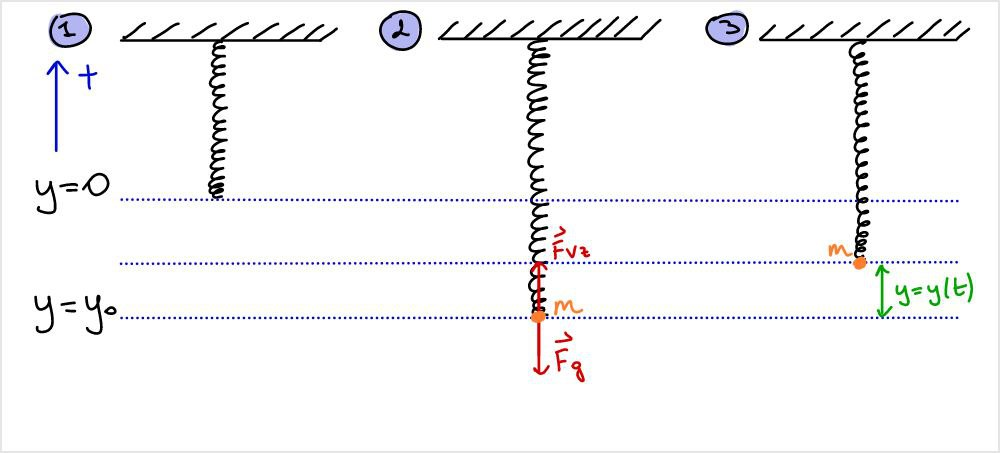
\includegraphics[width=0.7\textwidth]{img/01_001.jpg}      
\end{center}

\begin{enumerate}
    \item Vzmet je neraztegnjena.
    \item Obesimo vzmet z utežjo mase \(m\). Izračunamo \(y_0\) (ravnovesno lego):
    \begin{itemize}
        \item Zapišemo sile, ki delujejo na utež:
        \begin{enumerate}
            \item[(1)] Sila teže: \(\vec{F}_\text{g} = \vc{0}{-mg_0}{0}\), kjer je \(g_0 = 10 \, m / s^2\) težni pospešek;
            \item[(2)] Sila vzmeti: \(\vec{F}_\text{vz} = \vc{0}{-ky_0}{0}\), kjer je \(k > 0\) koeficient vzmeti.
        \end{enumerate}
        \item Zapišemo II.\ Newtonov zakon:
        \[
        \vec{a} = 0 \liff \vec{F} = m \vec{a} = 0 \lthen \vec{F}_\text{g} + \vec{F}_\text{vz} = 0.
        \]
        Torej
        \[
        -mg_0 - ky_0 = 0 \implies mg_0 = -ky_0 \implies y_0 = -\frac{mg_0}{k} \quad \textcolor{red}{(*)}
        \]        
    \end{itemize}
    \item Zdaj odmikamo utež od ravnovesne lege. Izračunamo spremembo \(y\)-koordinate v odvisnosti od časa \(y = y(t)\):
    \begin{itemize}
        \item Utež ima hitrost v smeri \(y\): \( v_y = \frac{dy}{dt} = \dot{y} = \neq 0\).
        \item Zapišemo sile, ki delujejo na utež:
        \begin{itemize}
            \item[(1)] Sila teže: \(\vec{F}_\text{g} = -mg_0 \widehat{e}_y\), kjer je \(\widehat{e}_y\) enotski vektor v smeri \(y\); 
            \item[(2)] Sila vzmeti: \(\vec{F}_\text{vz} = -ky\widehat{e}_y\);
            \item[(3)] Sila upora (linearni zakon upora, viskoznost): \(\vec{F}_\text{u} = -C \vec{v} = -C \dot{y} \widehat{e}_y\), kjer je \(C > 0\) \emph{koeficient upora}.
            \begin{itemize}
                \item Sila upora se pojavi, ker nismo v vakuumu.
            \end{itemize}            
        \end{itemize}
        \item Zapišemo II.\ Newtonov zakon:
        \begin{itemize}
            \item \(\vec{F} = \vec{F}_\text{g} + \vec{F}_\text{vz} + \vec{F}_\text{u}\);
            \item \(\vec{F} = m \vec{a} = m \ddot{y} \widehat{e}_y\).
        \end{itemize}
        Torej 
        \[
        -C \dot{y} \widehat{e}_y - ky\widehat{e}_y -mg_0 \widehat{e}_y = m \ddot{y} \widehat{e}_y \implies 
        \left( \ddot{y} + \frac{C}{m} \dot{y} + \frac{k}{m} y + g_0 \right) \widehat{e}_y = 0 \implies 
        \ddot{y} + \frac{C}{m} \dot{y} + \frac{k}{m} y + g_0 = 0.
        \]
        \item Vpeljemo oznake: \(\beta := \frac{C}{m}, \ [\beta]  = s^{-1}\) je \emph{koeficient dušenja}; in \( \omega_0^2 := \frac{k}{m}, \ [\omega_0^2] = s^{-2}\) je \emph{lastna frekvenca}. Dobimo enačbo:
        \[
        \ddot{y} + \beta \dot{y} + \omega_0^2 y + g_0 = 0.
        \]
        \item Iz \(\textcolor{red}{(*)}\) sledi, da \(g_0 = -\frac{k}{m}y_0 = - \omega_0^2y_0\).  
        \emph{Enačba dušenega nihanja} je:
        \[
        \boxed{\ddot{y} + \beta \dot{y} +  \omega_0^2 (y - y_0) = 0}
        \]        
    \end{itemize}
\end{enumerate}

\begin{opomba}
    Enačba \(\ddot{y} + \beta \dot{y} + \omega_0^2y = \omega_0^2 y_0\) je 
    \begin{itemize}
        \item Diferencialna enačba 2.\ reda za \(y\).
        \item Linearna (členi \(y, \ \dot{y}, \ \ddot{y}\) imajo 1.\ potenco).
        \item Koeficienti so konstantni (niso odvisni od časa).
        \item Pogojno nehomogena (lahko jo spravimo v homogeno enačbo).
    \end{itemize}
\end{opomba}

\paragraph{Postopek reševanja enačbe dušenega nihanja}
\begin{enumerate}
    \item Definiramo \(y' := y - y_0\) \emph{odmik od ravnovesne lege}. S tem enačba postane homogena.
    \item Enačbo rešujemo z nastavkov \(y' = A e^{\lambda t}\), kjer sta \(A, \ \lambda\) neki konstanti, \([\lambda] = s^{-1}, \ [A] = m\). 
    
    Dobimo karakteristični polinom \(\lambda^2 + \beta \lambda + \omega_0^2 = 0\).
    \item Karakteristični polinom ima diskriminanto \(D = \beta^2 - 4 \omega_0^2\). Definiramo \(\boxed{\omega^2 := \omega_0^2 - \left(\frac{\beta}{2}\right)^2}\). Dobimo \(D = - 4 \omega^2\). Ločimo možnosti.
\end{enumerate}

\textbf{(a) \(D < 0 \ (\omega^2 > 0)\)}. V tem primeru dobimo \emph{podkritično dušenje}.

Splošna rešitev (vsota dveh rešitev) je 
\[
    y' = \exp\left(-\frac{\beta}{2}t\right) (A_1 \exp(i\omega t) + A_2 \exp(-i\omega t)) = \exp\left(-\frac{\beta}{2}t\right)(B_1 \cos(\omega t) + B_2 \sin(\omega t)).
\]
Lahko jo zapišemo v obliki:
\[
    \boxed{y' = B \exp\left(-\frac{\beta}{2}t\right) \sin (\omega t + \delta)}
\]
kjer je \(\delta\) \emph{fazni zamik}.

\begin{primer}
    Če je \(\delta = 0\), potem \(y'(t) = B \exp (-\frac{\beta}{2} t) \sin (\omega t)\).
    \begin{figure}[h!]
        \centering
        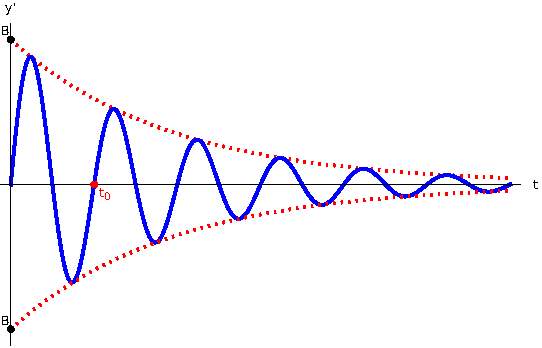
\includegraphics[width=0.7\textwidth]{img/01_002.pdf}
        \caption{Dušeno nihanje v primeru podkritičnega dušenja}      
    \end{figure}
    
    Definiramo količine:
    \begin{itemize}
        \item \(t_0 = \frac{2pi}{\omega}\) je \emph{nihajni čas} (čas enega nihaja).
        \item \(\nu = \frac{1}{t_0}\) je \emph{frekvenca}.
        \begin{itemize}
            \item \(\nu = \frac{1}{t_0} = \frac{\omega}{2 \pi} \lthen \boxed{\omega = 2 \pi \nu}\)
        \end{itemize}
    \end{itemize}

    Če je dušenje zelo šibko, potem \(\left(\ds \frac{\beta}{2}\right)^2 \ll w_0^2 \lthen t_0 \approx \frac{2 \pi}{\sqrt{\omega_0^2}} = 2 \pi \sqrt{\frac{m}{k}}\)
\end{primer}

\paragraph{Kako dobimo parametri \(B\) in \(\delta\)?} Iz začetnih pogojev! Na primer:
\begin{itemize}
    \item \(y'(0) = a\) odmik od ravnovesne lege v času \(t = 0\);
    \item \(\dot{y'}(0) = b\) hitrost v času \(t = 0\).
\end{itemize}
Rešimo enostaven sistem enačb in definiramo \(\ds r:= \frac{a}{b}\), potem \(\boxed{\delta = \arctan \left(\frac{r \omega}{1+\frac{r\beta}{2}}\right)}\) in \(\boxed{B = \frac{|b|}{\omega}}\)

\newpage
\textbf{(b) \(D = 0 \ (\omega = 0)\)}. V tem primeru dobimo \emph{kritično dušenje}.

Rešitvi sta \(y_1' = B_1 \exp \left(-\frac{\beta}{2}t\right)\) in \(y_2' = B_2 t \exp \left(-\frac{\beta}{2}t\right)\). Splošna rešitev je 
\[\boxed{(B_1 + B_2t) \exp \left(-\frac{\beta}{2} t\right)}\]

\begin{opomba}
    Opazimo, da nihanja sploh ni.
\end{opomba}

\begin{figure}[h!]
    \centering
    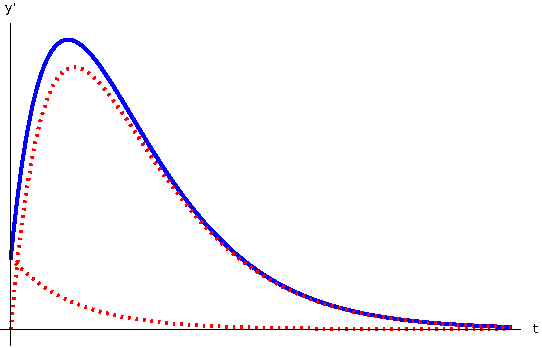
\includegraphics[width=0.7\textwidth]{img/01_003.pdf}
    \caption{Dušeno nihanje v primeru kritičnega dušenja}      
\end{figure}

\textbf{(c) \(D > 0 \ (\omega^2 < 0)\)}. V tem primeru dobimo \emph{nadkritično dušenje}. 

Splošna rešitev je 
\[
\boxed{y' = B_1 \exp \left(- \frac{\beta}{2} \left[1 + \sqrt{1 - \frac{4 \omega_0^2}{\beta^2}}\right]t\right) + B_2 \exp \left(- \frac{\beta}{2} \left[1 - \sqrt{1 - \frac{4 \omega_0^2}{\beta^2}}\right]t\right)} 
\]

\begin{opomba}
    Rešitev je vsota dveh eksponentno padajočih prispevkov (nihanja ni).
\end{opomba}

V primeru zelo močnega dušenja \((\frac{4\omega_0^2}{\beta^2} \ll 1)\) velja, da \(\sqrt{1 - \frac{4 \omega_0^2}{\beta^2}} \approx 1 - \frac{2\omega_0^2}{\beta^2}\). V tem primeru 
\[
y' = C_1 \exp (-\beta t) + C_2 \exp \left(-\frac{\beta}{2} \frac{2 \omega_0^2}{\beta^2}t\right)
\]

\begin{itemize}
    \item Prvi člen: zelo hitro padanje k ničli (hitreje, kot pri kritičnem dušenju);
    \item Drugi člen: zelo počasno približanje ravnovesni legi!
\end{itemize}

\subsubsection*{Energija nihala}
Posamezni prispevki energije:
\begin{itemize}
    \item \(W_\text{k} = \frac{1}{2}mv^2, \ v = v_y = \dot{y} = \dot{(y - y_0)} = \dot{y'} \lthen W_\text{k} = \frac{1}{2}m (\dot{y'})^2\)
    \item \(W_\text{pr} = \frac{1}{2}ky^2 = \frac{1}{2}(y' + y_0)^2\)
    \item \(W_\text{p} = mg_0(y'+y_0)\)
\end{itemize}

Torej \(\boxed{W = W_\text{k} + W_\text{pr} + W_\text{p}}\)

\paragraph{\(W\) za zelo šibko dušenje \(\left(\frac{\beta}{2}t \ll 1\right)\):}

\(\left(\frac{\beta}{2}\right)^2 \ll \omega_0^2 \lthen \omega \approx \omega_0 = \sqrt{\frac{k}{m}}\).

Z enostavnim računom dobimo, da \[\boxed{W = \frac{1}{2}kB^2 + \frac{1}{2}ky_0^2 + mg_0y_0 = \text{const}}\]

\paragraph{\(W\) za nihanje z dušenjem:} \todo{DN}

\newpage
\subsubsection*{Nitno (matematično) nihalo}
\begin{wrapfigure}{l}{0.4\textwidth}
    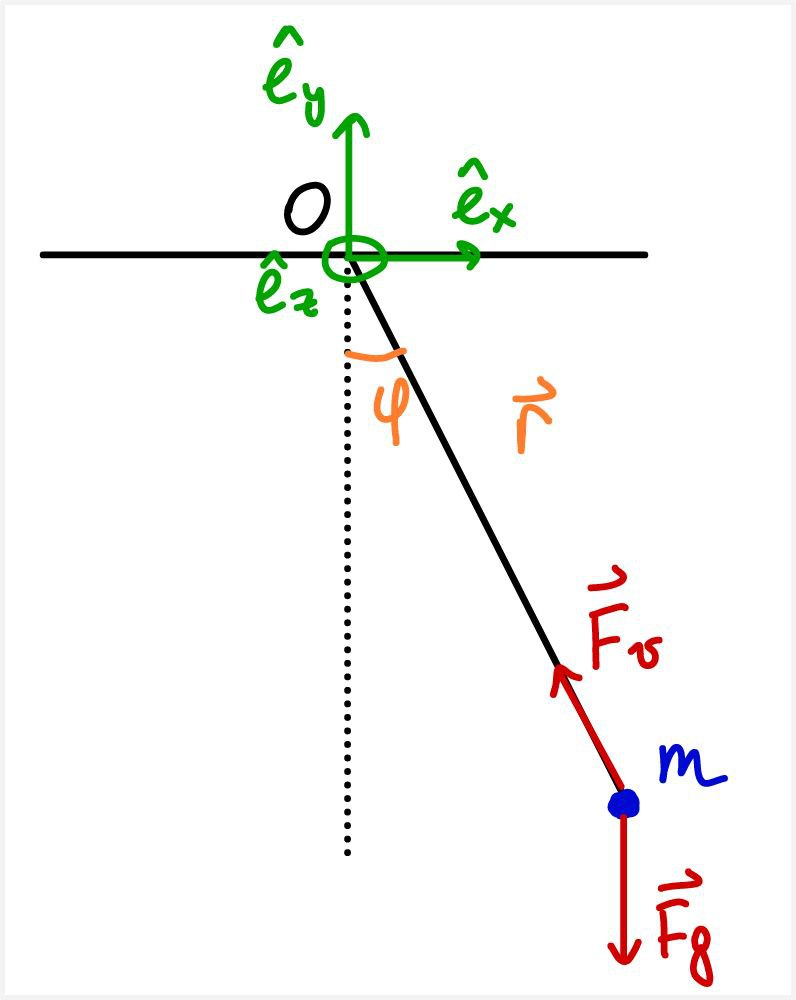
\includegraphics[width=0.9\linewidth]{img/01_004.jpg} 
\end{wrapfigure}
Naj bo \(|\vec{r}| = l\). 
\begin{enumerate}
    \item Izračunamo navor \(\vec{M} = \vec{r} \times (\sum \vec{F})\) na točkasto telo z maso \(m\). Dobimo: \(\vec{M} = (0, 0, -mgl \sin \phi)\).
    \item Zapišemo II.\ Newtonov zakon za vrtenje okoli fiksne osi \(\hat{e}_z\): 
    \[M_z = J_z  \alpha = ml^2  \ddot{\phi}\]
    \item Dobimo enačbo \[\boxed{\ddot{\phi} + \frac{g_0}{l} \sin \phi = 0}\]
\end{enumerate}

\begin{opomba}
    V splošnem to ni enačba sinusnega nihanja. 
\end{opomba}

Če je \(\phi \ll 1\), potem \(\sin \phi \approx \phi\). V tem primeru dobimo enačbo:
\[\boxed{\ddot{\phi} + \omega_0^2 \phi = 0}\]
ki ima rešitev \(\phi(t) = B \sin(w_0t + \delta)\), kjer \(\ds \omega_0 = \sqrt{\frac{g_0}{l}}\). Od tod dobimo, da je 
\begin{itemize}
    \item \(\ds t_0 = \frac{2 \pi}{\omega} = 2 \pi \sqrt{\frac{l}{g_0}}\)
\end{itemize}
\ 
\\

\subsubsection*{Energija matematičnega nihala}
Preprost račun pokaže, da 
\[\boxed{W = W_\text{k} + W_\text{p} = -mg_0l(1 - \frac{1}{2}B^2) = \text{const}}\]

\begin{opomba}
    Ohranitev \(W = W_\text{k} + W_\text{p}\) velja tudi, ko \(\phi \not \ll 1\).
\end{opomba}

\subsubsection*{Fizična nihala}
\begin{wrapfigure}{l}{0.4\textwidth}
    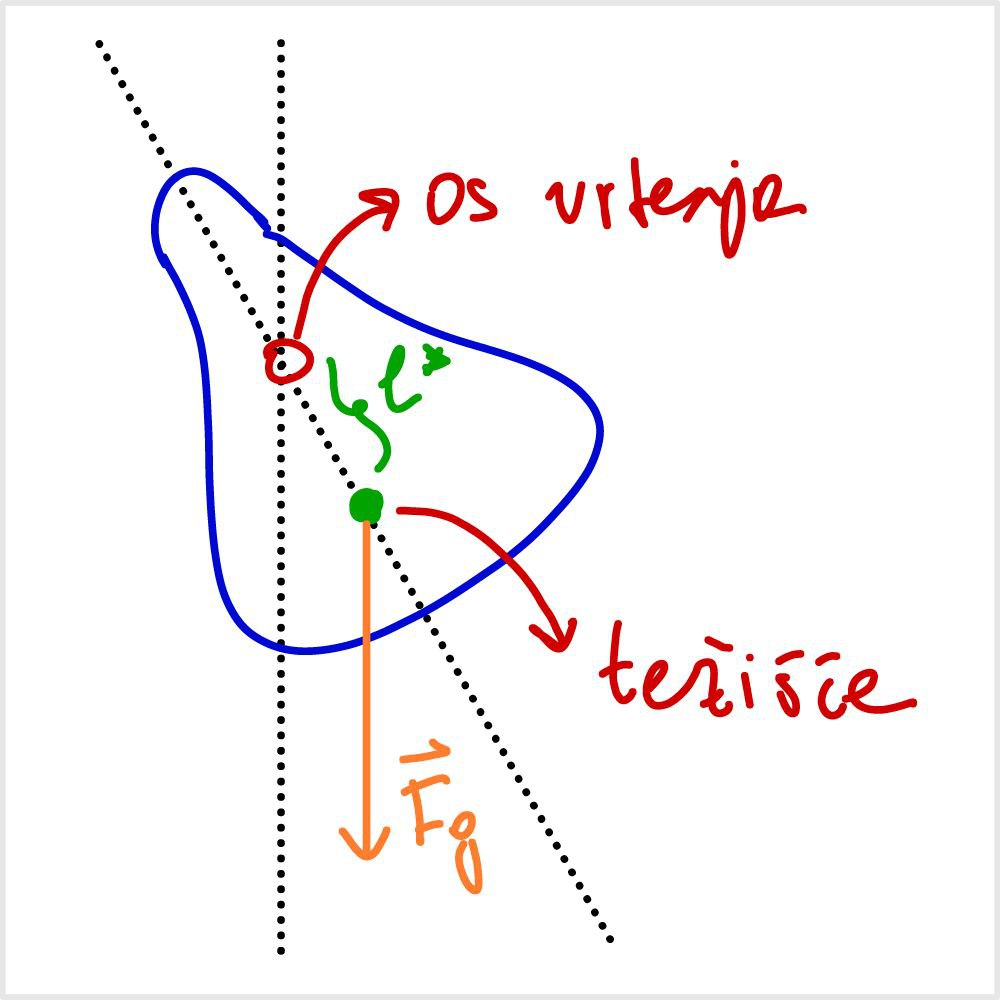
\includegraphics[width=0.9\linewidth]{img/01_005.jpg} 
\end{wrapfigure}
Naj bo \(l^*\) razdalja med osjo vrtenja in težiščem. Potem 
\[M_z = -mgl^* \sin \phi \quad \text{in} \quad M_z = J_z \alpha,\]
kjer je \(J_z\) vztrajnostni moment telesa pri vrtenju okoli dane osi (izračunamo ga z uporabo Steinerjevega izreka).

Dobimo enačbo nedušenega nihanja
\[
\boxed{\ddot{\phi} + \frac{mgl^*{J_z}}\phi = 0}
\]
Iz njo dobimo
\begin{itemize}
    \item \(\omega_0^2 = \frac{mgl^*}{J_z}\)
    \item \(t_0 = \frac{2 \pi}{\omega_0} = 2 \pi \sqrt{\frac{J_z}{mgl^*}}\)
\end{itemize}
\ 
\\ 
\\ 
\\
\\
\newpage
\subsubsection*{Nihalo na vijačnih vzmeteh na zračni klopi}
\begin{figure}[h!]
    \centering
    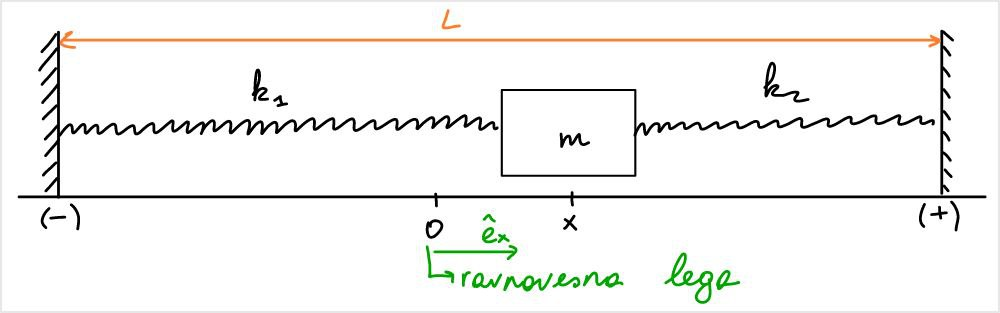
\includegraphics[width=0.7\textwidth]{img/01_006.jpg}  
\end{figure}

\begin{itemize}
    \item Naj bo \(l_{1, 0}\) začetna dolžina 1.\ vzmeti
    \item Naj bo \(l_{1, r}\) dolžina 1.\ vzmeti, ko je telo v ravnovesni legi.    
    \item Naj bo \(\Delta l_{1, r} = l_{1, r} - l_{1, 0}\) raztezek ali skrček 1.\ vzmeti, ko je telo v ravnovesni legi.
\end{itemize}
Zapišemo sili, ki delujejo na telo v ravnovesni legi:
\begin{itemize}
    \item \(\vec{F}_{1, r} = -k_1 \Delta l_{1, r} \hat{e}_x\) je sila 1.\ vzmeti 
    \item \(\vec{F}_{2, r} = +k_2 \Delta l_{2, r} \hat{e}_x\) je sila 2.\ vzmeti 
\end{itemize}
Zapišemo II.\ Newtonov zakon v ravnovesju:
\[
\vec{F}_r = \vec{F}_{1, r} + \vec{F}_{2, r} + \vec{F}_g + \vec{F}_N = \vec{F}_{1, r} + \vec{F}_{2, r} = 0 \lthen \frac{\Delta l_{1, r}}{\Delta l_{2, r}} = \frac{k_2}{k_1}
\]
Zapišemo II.\ Newtonov zakon v legi \(x\):
\begin{itemize}
    \item \(\Delta l_1 = \Delta l_{1, r} + x\) in \(\Delta l_2 = \Delta l_{2, r} - x\) 
    \item \(\vec{F_1} = -k_1 \Delta l_1 \hat{e}_x = \vec{F}_{1, r} - k_1x\hat{e}_x\) in \(\vec{F_2} = +k_2 \Delta l_2 \hat{e}_x = \vec{F}_{2, r} - k_2x\hat{e}_x\)
\end{itemize}
Dobimo enačbo 
\[
\boxed{\ddot{x} + \frac{k_1 + k_2}{m} x = 0}
\]

Iz njo dobimo:
\begin{itemize}
    \item \(\omega_0^2 = \frac{k_1 + k_2}{m}\)
    \item \(t_0 = 2 \pi \sqrt{\frac{m}{k_1 + k_2}}\)
\end{itemize}

\subsection{Vsiljeno (dušeno) nihanje}
Delujemo z dodatno \(\nu = \frac{1}{t_v}\) frekvenco vsiljevanja na našo nihalo \((\omega_v = 2 \pi \nu_v)\). Naj bo dodatna sila \(\vec{F_y} = F_0 \sin(\omega_v t) \hat{e}_y\).

Zanima nas, kaj je \(y(t)\)? Enačba gibanja je 
\[
\boxed{\ddot{y} + \beta \dot{y} + \omega_0^2(y-y_0) = \frac{F_0}{m} \sin(\omega_vt)}
\]

\begin{opomba}
    Ta enačba je nehomogena!
\end{opomba}

Postopek reševanja:
\begin{enumerate}
    \item Naredimo substitucijo \(y' = y - y_0\). Dobimo enačbo \(\ddot{y'} + \beta \dot{y'} + \omega_0^2y' = \frac{F_0}{m} \sin(\omega_vt)\)
    \item Najbolj splošna rešitev je oblike \(y' = y'_h + y'_p\), kjer je \(y'_h\) rešitev homogenega dela in \(y'_p\) neka partikularna rešitev
\end{enumerate}

Rešitev homogenega dela (za podkritično dušenje) že poznamo: \[y'_h = B \exp\left(- \frac{\beta}{2}t\right) \sin(\omega t + \delta_h),\]
kjer \(\omega = \sqrt{\omega_0^2 - \left(\frac{\beta}{2}\right)^2}\).

Opazimo, za da čase \(t \gg \frac{1}{\beta}\): \(y'_h \to 0\). Takrat bo rešitev
\[
\boxed{y' \approx y'_p = B_p \sin(\omega_v t - \delta_p)}
\]
kjer \(B_p > 0\).

\begin{opomba}
    Za dovolj velike čase bo frekvenca \(\omega_v\) namesto \(\omega\).
\end{opomba}

\newpage
\subsection{Sklopljeno nihanje}
\begin{figure}[h!]
    \centering
    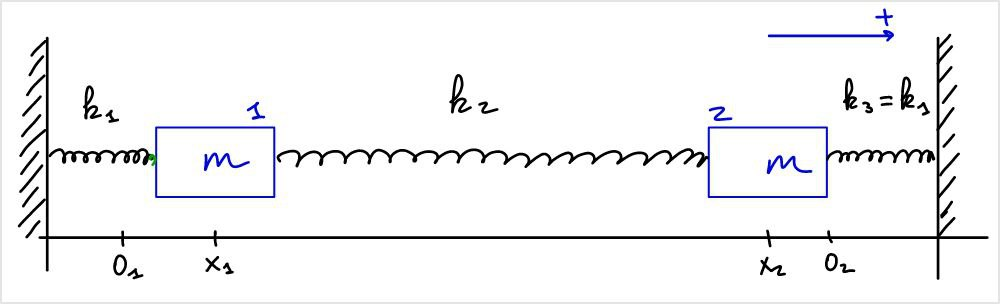
\includegraphics[width=0.7\textwidth]{img/01_007.jpg}  
\end{figure}
Predpostavimo, da dušenja ni. Za začetek rešimo simetrični problem:
\begin{itemize}
    \item \(m_1 = m_2 = m\)
    \item \(k_1 = k_3\)
\end{itemize}
Dobimo enačbi gibanja:
\[
\boxed{\ddot{x}_1 + \omega_1^2 x_1 + \omega_2^2(x_1 - x_2) = 0 \quad \text{in} \quad \ddot{x}_2 + \omega_1^2x_2 - \omega_2^2(x_1 - x_2) = 0} 
\]
kjer \(\omega_1^2 = \frac{k_1}{m}\) in \(\omega_2^2 = \frac{k_2}{m}\).

Rešitvi sta 
\[
\boxed{x_1 = B_1 \sin(\omega_at + \delta_a) + B_2 \sin(\omega_bt + \delta_b) \quad \text{in} \quad x_2 = B_1 \sin(\omega_at + \delta_a) - B_2 \sin(\omega_bt + \delta_b)}
\]
kjer \(\omega_a = \omega_1\) in \(\omega_b = \sqrt{\omega_1^2 + 2\omega_2^2}\).

Konstanti \(B_1, \ B_2, \ \delta_a, \ \delta_b\) dobimo iz začetnih pogojev (položaji in hitrosti nihal ob času \(t = 0\)).

\subsubsection*{Lastno nihanje sestavljenega nihala}
\todo{Poglavje}

\newpage
\subsection{Mehansko valovanje - valovna enačba}
\subsubsection*{Valovanje po vijačni vzmeti}
\begin{itemize}
    \item Poskus: valovanje - širjenje motnje (def.) po vijačni vzmeti
    \item Model masivne vzmeti: veliko število drobnih mas, povezanih z neskončno lahkimi vijačnimi vzmetmi (sklopljena vzmetna nihala)
\end{itemize}
\begin{figure}[h!]
    \centering
    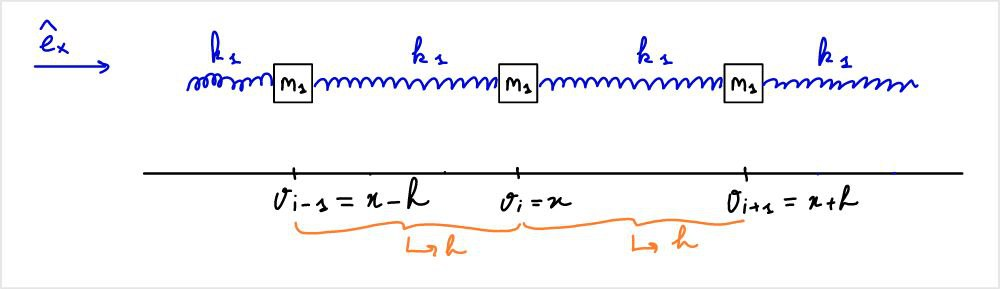
\includegraphics[width=0.8\textwidth]{img/01_008.jpg}  
\end{figure}

Začetna situacija:
\begin{itemize}
    \item Masa celotne vzmeti: \(m\)
    \item Koeficient vzmeti: \(k\)
    \item Dolžina vzmeti: \(l\)
\end{itemize}

Razbijemo na \(n\) majhnih delov:
\begin{itemize}
    \item Število uteži: \(n\)
    \item Masa eni uteži: \(m_1 \frac{m}{n}\)
    \item Razdalja med dvema uteži v ravnovesju: \(h = \frac{l}{n} \liff n = \frac{l}{h}\)
    \item Koeficient vzmeti med uteži: \(k_1 = kn = k \frac{l}{h}\)
    \item Ravnovesna lega \(i\)-te uteži: \(x\)
\end{itemize}

Kaj se dogaja izmed ravnovesja?
\begin{figure}[h!]
    \centering
    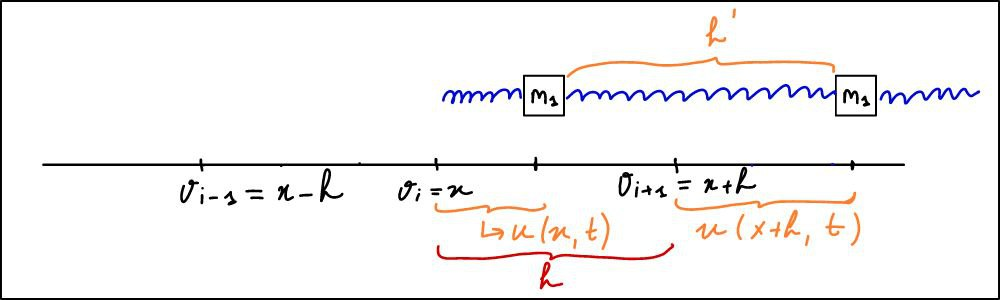
\includegraphics[width=0.7\textwidth]{img/01_009.jpg}  
\end{figure}
\begin{itemize}
    \item Označimo z \(u(x, t)\) odmik uteži, ki je v ravnovesni legi na položaju \(x\), od ravnovesne lege v času \(t\)
    \begin{itemize}
        \item Podobno definiramo: \(u(x - h, t)\), \(u(x + h, t)\) itn.
    \end{itemize}
    \item Vsi odmiki so v smeri \(\hat{e}_x\)
    \item \(x \neq x(t)\), tj. vzmet se ne premika sleda, da ravnovesne lege se ne premika
    \begin{itemize}
        \item Tudi \(\dot{x} = 0\)
    \end{itemize}
    \item \(u(x, t) + h' = h + u(x+h, t) \lthen \Delta h = h' - h  = u(x + h, t) - u(x, t)\)
\end{itemize}
%
Zdaj bi radi zapisali Newtonov zakon na \(i\)-ti utež. Dobimo:
\[
\sum F_i = kl \cdot  \frac{u(x+h, t) - 2u(x, t) + u(x -h, t)}{h}
\]
%
Po drugi strani:
\[
F_i = m_1 \cdot \frac{d^2u(x, t)}{dt^2} = m_1 \cdot \frac{\partial^2 u}{\partial t^2} = \frac{m}{n}h \frac{\partial^2 u}{\partial t^2}
\]
%
\emph{Newtonov zakon za \(i\)-ti utež} je torej
%
\[
    \frac{\partial^2 u}{\partial t^2} = \frac{kl^2}{m} \cdot \frac{u(x+h, t) - 2u(x, t) + u(x -h, t)}{h^2}
\]
\newpage
%
Če \(n \to \infty\), potem \(h = \frac{l}{n} \to 0\). Dobimo 
%
\[
\frac{\partial^2u(x,t)}{\partial x^2} = \lim_{h \to 0} \frac{u(x+h, t) - 2u(x, t) + u(x -h, t)}{h^2} \ \textcolor{red}{(*)}
\]
%
\(\ds \frac{\partial^2u(x,t)}{\partial x^2}\) imenujemo \emph{drugi simetrični odvod} \(u\) po \(x\). Ta odvod je enak limiti na desni v izrazu \textcolor{red}{(*)}, če obstaja.

Torej v limiti dobimo enačbo
%
\[
    \boxed{\frac{\partial^2 u(x, t)}{\partial t^2} = C^2 \frac{\partial^2u(x,t)}{\partial x^2}}
\]
%
kjer \(\ds C^2 = \frac{kl^2}{m}\). Tej enačbe pravimo \emph{valovna enačba}.
\begin{itemize}
    \item \([C^2] = \frac{\text{m}^2}{\text{s}^2} \lthen [C] = \frac{\text{m}}{\text{s}}\). \(C\) je \emph{hitrost valovanja}.
\end{itemize}

\subsubsection*{Valovanje v tekočini, zaprti v tanki togi cevi}
\begin{itemize}
    \item Viskoznost: \(\eta \to 0\), tj. ni sil med tekočino in steno
    \item \(S = \text{const}\), tj. cev je toga
    \item Stisljivost tekočine: \(\chi \)  
\end{itemize}
%
Velja:
%
\[
\Delta p = - \frac{1}{\chi} \frac{\Delta V}{V} \ \text{(sprememba tlaka)} \lthen \frac{\Delta F}{S} = - \frac{1}{\chi} \frac{S \Delta l}{S l} \lthen \Delta F = - \frac{S}{\chi l} \Delta l
\]
%
Če definiramo \(k = \frac{S}{\chi l}\), dobimo zvezo \(\Delta F = -k \Delta l\), ke je podobna Hookovemu zakonu. Torej tekočino lahko obravnavamo kot vzmet!

Po istem postopku dobimo valovno enačbo, pri čemer
%
\[
C^2 = \frac{kl^2}{m} = \frac{Sl^2}{\chi l m} = \frac{Sl}{\chi m} = \frac{V}{\chi m} = \frac{1}{\chi \rho} \lthen C^2 = \frac{1}{\chi \rho}
\]

\subsubsection*{Valovanje po elastični palici}
\begin{itemize}
    \item Elastični modul: \(E\)
    \begin{itemize}
        \item \([E] = \frac{\text{N}}{\text{m}^2}\)
        \item \(\frac{\Delta F}{S} = -E \frac{\Delta l}{l}\)
    \end{itemize}
\end{itemize}

Če definiramo \(k = \frac{ES}{l}\), dobimo \(\Delta F = -k \Delta l\).

Spet uporabimo isti matematični model, dobimo isto enačbo, kjer
\[
C^2 = \frac{kl^2}{m} = \frac{ESl^2}{lm} = \frac{ESl}{m} = \frac{EV}{m} = \frac{E}{\rho} \lthen C^2 = \frac{E}{\rho}
\]